% **************************************************************************************************
% ** SPSC Report and Thesis Template
% **************************************************************************************************
%
% ***** Authors *****
% Daniel Arnitz, Paul Meissner, Stefan Petrik
% Signal Processing and Speech Communication Laboratory (SPSC)
% Graz University of Technology (TU Graz), Austria
%
% ***** Changelog *****
% 0.1   2010-01-25   extracted from report template by Daniel Arnitz (not ready yet)
% 0.2   2010-02-08   added thesis titlepage and modified layout (not ready yet)
% 0.3   2010-02-18   added TUG logo and statutory declaration
% 0.4   2010-02-18   moved the information fields below % **************************************************************************************************
% ** SPSC Report and Thesis Template
% **************************************************************************************************
%
% ***** Authors *****
% Daniel Arnitz, Paul Meissner, Stefan Petrik
% Signal Processing and Speech Communication Laboratory (SPSC)
% Graz University of Technology (TU Graz), Austria
%
% ***** Changelog *****
%
% ***** Todo *****
%
% **************************************************************************************************



\documentclass[%
a4paper,% !!! ATTENTION: geometry package below !!!
\Twosided,% !!! ATTENTION: geometry package below !!!
openany,% begin chapters with new right page (openright) or don't care (openany)
11pt,%
fleqn,% equations not centered, but on the left side
tablecaptionbelow,% captions below tables
% titlepage,% use title
pointlessnumbers,% do not generate point at the end of section numbers (e.g. 1.4.5 instead of 1.4.5.)
final,%
]{scrreprt}% (KOMA)

\usepackage[paper=a4paper,\Twosided,%
textheight=246mm,%
textwidth=160mm,%
heightrounded=true,% round textheight to multiple of lines (avoids overfull vboxes)
ignoreall=true,% do not include header, footer, and margins in calculations
marginparsep=5pt,% marginpar only used for signs (centered), thus only small sep. needed
marginparwidth=10mm,% prevent margin notes to be out of page
hmarginratio=2:1,% set margin ration (inner:outer for twoside) - (2:3 is default)
]{geometry}%


% master
\usepackage{ifthen}% for optional parts
\usepackage[latin1]{inputenc}% German special characters
\ifthenelse{\equal{\DocumentLanguage}{en}}{\usepackage[USenglish]{babel}}{}%
\ifthenelse{\equal{\DocumentLanguage}{de}}{\usepackage[ngerman]{babel}}{}%
\usepackage[%
headtopline,plainheadtopline,% activate all lines (header and footer)
headsepline,plainheadsepline,%
footsepline,plainfootsepline,%
footbotline,plainfootbotline,%
automark% auto update \..mark
]{scrpage2}% (KOMA)
\usepackage{makeidx}% used to make an index directory
\usepackage[]{caption}% customize captions
\usepackage{multicol}%
\usepackage[stable,bottom,hang,splitrule,multiple,symbol*]{footmisc}% customize footnotes


% text
\usepackage{varioref}% improved references
\usepackage{color}% e.g., for color boxes
\usepackage{rotating}% to rotate objects
\usepackage{gensymb}% symbols (perthousand, Celsius, ...)
\usepackage[right]{eurosym}% euro symbol on the right side (51 EUR)
\usepackage[normalem]{ulem}% cross-out, strike-out, underlines (normalem: keep \emph italic)
%\usepackage[safe]{textcomp}% loading in safe mode to avoid problems (see LaTeX companion)
%\usepackage[geometry,misc]{ifsym}% technical symbols
\usepackage{remreset}%\@removefromreset commands (e.g., for continuous footnote numbering)
\usepackage[%
breaklinks=true,% allow line break in links
colorlinks=true,% if false: framed link
linkcolor=black,anchorcolor=black,citecolor=black,filecolor=black,%
menucolor=black,urlcolor=black]{hyperref}% hyperlinks for references


% math
\usepackage{amsmath,amssymb,amstext,bm} % use math packages
\usepackage{mathcomp}% symbols (perthousand, ...) in math mode


% graphics
\usepackage{graphicx}% use simple graphics
\usepackage{subfigure}% subfigures (a),(b),(c)... within figures
\usepackage{flafter}% place floats always after reference
\usepackage{placeins}% preventing floats from crossing a barrier
\usepackage{float}% to place floats !HERE!
\usepackage{psfrag}% replace text in eps figures


% tables
\usepackage{hhline}% hline doesn't work with colored columns, so using hhline
\usepackage{longtable}% for tables longer than one page
\usepackage{dcolumn}% for number alignment in tables
\usepackage{colortbl}% color in tables


% listings
%\usepackage{alltt}% verbatim environment with commands available
\usepackage{listings}% program code listings


% other
%\usepackage{layout}% graphical page layout (spacings)
\usepackage{xspace}% add space after macros if not followed by punctuation character
\makeindex% used for index creation

 (encoding...)
% 0.5   2010-03-02   added \ShortTitle to fix problems with long thesis titles
%                    added \ThesisType (makes the template suitable for MSc, BSc, PhD, ... Thesis)
%
% ***** Todo *****
% - Introduction/Usage
% **************************************************************************************************

% **************************************************************************************************
% basic setup
\newcommand{\DocumentType}{report} % "thesis" / "report"
\newcommand{\DocumentLanguage}{en} % "en" / "de"
\newcommand{\Twosided}{} % "twoside" / ""


% **************************************************************************************************
% template setup -- do not change these unless you know what you are doing!
% **************************************************************************************************
% ** SPSC Report and Thesis Template
% **************************************************************************************************
%
% ***** Authors *****
% Daniel Arnitz, Paul Meissner, Stefan Petrik
% Signal Processing and Speech Communication Laboratory (SPSC)
% Graz University of Technology (TU Graz), Austria
%
% ***** Changelog *****
%
% ***** Todo *****
%
% **************************************************************************************************



\documentclass[%
a4paper,% !!! ATTENTION: geometry package below !!!
\Twosided,% !!! ATTENTION: geometry package below !!!
openany,% begin chapters with new right page (openright) or don't care (openany)
11pt,%
fleqn,% equations not centered, but on the left side
tablecaptionbelow,% captions below tables
% titlepage,% use title
pointlessnumbers,% do not generate point at the end of section numbers (e.g. 1.4.5 instead of 1.4.5.)
final,%
]{scrreprt}% (KOMA)

\usepackage[paper=a4paper,\Twosided,%
textheight=246mm,%
textwidth=160mm,%
heightrounded=true,% round textheight to multiple of lines (avoids overfull vboxes)
ignoreall=true,% do not include header, footer, and margins in calculations
marginparsep=5pt,% marginpar only used for signs (centered), thus only small sep. needed
marginparwidth=10mm,% prevent margin notes to be out of page
hmarginratio=2:1,% set margin ration (inner:outer for twoside) - (2:3 is default)
]{geometry}%


% master
\usepackage{ifthen}% for optional parts
\usepackage[latin1]{inputenc}% German special characters
\ifthenelse{\equal{\DocumentLanguage}{en}}{\usepackage[USenglish]{babel}}{}%
\ifthenelse{\equal{\DocumentLanguage}{de}}{\usepackage[ngerman]{babel}}{}%
\usepackage[%
headtopline,plainheadtopline,% activate all lines (header and footer)
headsepline,plainheadsepline,%
footsepline,plainfootsepline,%
footbotline,plainfootbotline,%
automark% auto update \..mark
]{scrpage2}% (KOMA)
\usepackage{makeidx}% used to make an index directory
\usepackage[]{caption}% customize captions
\usepackage{multicol}%
\usepackage[stable,bottom,hang,splitrule,multiple,symbol*]{footmisc}% customize footnotes


% text
\usepackage{varioref}% improved references
\usepackage{color}% e.g., for color boxes
\usepackage{rotating}% to rotate objects
\usepackage{gensymb}% symbols (perthousand, Celsius, ...)
\usepackage[right]{eurosym}% euro symbol on the right side (51 EUR)
\usepackage[normalem]{ulem}% cross-out, strike-out, underlines (normalem: keep \emph italic)
%\usepackage[safe]{textcomp}% loading in safe mode to avoid problems (see LaTeX companion)
%\usepackage[geometry,misc]{ifsym}% technical symbols
\usepackage{remreset}%\@removefromreset commands (e.g., for continuous footnote numbering)
\usepackage[%
breaklinks=true,% allow line break in links
colorlinks=true,% if false: framed link
linkcolor=black,anchorcolor=black,citecolor=black,filecolor=black,%
menucolor=black,urlcolor=black]{hyperref}% hyperlinks for references


% math
\usepackage{amsmath,amssymb,amstext,bm} % use math packages
\usepackage{mathcomp}% symbols (perthousand, ...) in math mode


% graphics
\usepackage{graphicx}% use simple graphics
\usepackage{subfigure}% subfigures (a),(b),(c)... within figures
\usepackage{flafter}% place floats always after reference
\usepackage{placeins}% preventing floats from crossing a barrier
\usepackage{float}% to place floats !HERE!
\usepackage{psfrag}% replace text in eps figures


% tables
\usepackage{hhline}% hline doesn't work with colored columns, so using hhline
\usepackage{longtable}% for tables longer than one page
\usepackage{dcolumn}% for number alignment in tables
\usepackage{colortbl}% color in tables


% listings
%\usepackage{alltt}% verbatim environment with commands available
\usepackage{listings}% program code listings


% other
%\usepackage{layout}% graphical page layout (spacings)
\usepackage{xspace}% add space after macros if not followed by punctuation character
\makeindex% used for index creation


\input{./base/layout_\DocumentType}
% **************************************************************************************************
% ** SPSC Report and Thesis Template
% **************************************************************************************************
%
% ***** Authors *****
% Daniel Arnitz, Paul Meissner, Stefan Petrik
% Signal Processing and Speech Communication Laboratory (SPSC)
% Graz University of Technology (TU Graz), Austria
%
% ***** Changelog *****
%
% ***** Todo *****
%
% **************************************************************************************************



% **************************************************************************************************
% * SECTIONING AND TEXT
% **************************************************************************************************

% new chapter, section, ... plus a few addons
%   part
\newcommand{\newpart}[2]{\FloatBarrier\cleardoublepage\part{#1}\label{part:#2}}%
%   chapter
\newcommand{\newchapter}[2]{\FloatBarrier\chapter{#1}\label{chp:#2}}
\newcommand{\newchapterNoTOC}[2]{\FloatBarrier\stepcounter{chapter}\chapter*{#1}\label{chp:#2}}%
%   section
\newcommand{\newsection}[2]{\FloatBarrier\vspace{5mm}\section{#1}\label{sec:#2}}%
\newcommand{\newsectionNoTOC}[2]{\FloatBarrier\vspace{5mm}\stepcounter{section}\section*{#1}\label{sec:#2}}%
%   subsection
\newcommand{\newsubsection}[2]{\FloatBarrier\vspace{3mm}\subsection{#1}\label{sec:#2}}%
\newcommand{\newsubsectionNoTOC}[2]{\FloatBarrier\vspace{3mm}\stepcounter{subsection}\subsection*{#1}\label{sec:#2}}%
%   subsubsection
\newcommand{\newsubsubsection}[2]{\vspace{2mm}\subsubsection{#1}\label{sec:#2}}%
\newcommand{\newsubsubsectionNoTOC}[2]{\vspace{2mm}\stepcounter{subsubsection}\subsubsection*{#1}\label{sec:#2}}%

% next paragraph
\newcommand{\nxtpar}{\par\bigskip}

% "stylish" quotes on the right side
\newcommand{\openingquote}[2]{\hfill\parbox[t]{10cm}{\itshape\raggedleft{"#1"}\\\footnotesize -- #2}\nxtpar}%

% direct quotes
% \newenvironment{directquote}{\nxtpar\hrule}{\hrule}\hfill\litref{#1}{#2}}

% warnings and attention signs in marginpar
\newcommand{\MDanger}{\marginpar{\Huge\centering\fbox{\textbf{!}}}}%
\newcommand{\MAttention}{\marginpar{\Huge\centering\textbf{!}}}%
\newcommand{\MHint}{\marginpar{\Huge\centering\textbf{\checkmark}}}%
\newcommand{\MQuestion}{\marginpar{\Huge\centering\textbf{?}}}%

% same footnote number as last one
\newcommand{\lastfootnotemark}{\addtocounter{footnote}{-1}\footnotemark}%

% value-unit commands (for 457 kHz, etc)
\newcommand{\vu}[2]{\mbox{$#1\,\text{#2}$}} % "value~unit" ... prevents e.g. 456 \linebreak mV
\newcommand{\vuc}[3]{\mbox{$#1\,\text{#2}\;#3\,\%$}} % "value~unit~tolerance-per-cent"
\newcommand{\vum}[3]{\mbox{$#1\,\text{#2}\;#3\,\perthousand$}} % "value~unit~tolerance-per-mil"

% reminders
\newcommand{\reminder}[1]{\colorbox{red}{#1}\xspace}%
\newcommand{\rem}{\reminder{(...)}}%
\newcommand{\remq}{\reminder{???}}%
\newcommand{\uc}{\nxtpar\colorbox{yellow}{... under construction ...}\nxtpar}%

% misc
\newcommand{\pwd}{.} % present working directory (can be used to create relativ paths per part, etc.)


% **************************************************************************************************
% * MATH
% **************************************************************************************************

% highlighting
\newcommand{\vm}[1]{\bm{#1}}% vector or matrix

% operators
\newcommand{\E}[1]{\text{E}\!\left\{#1\right\}}% expectation operator
\newcommand{\var}[1]{\text{var}\!\left\{#1\right\}}% variance operator
\renewcommand{\ln}[1]{\text{ln}\!\left(#1\right)}% natural logarithm
\newcommand{\ld}[1]{\text{ld}\!\left(#1\right)}% logarithm base 2
\renewcommand{\log}[1]{\text{log}\!\left(#1\right)}% logarithm (base 10)
\newcommand{\logb}[2]{\text{log}_{#1}\!\left(#2\right)}% logarithm base ...
\newcommand{\avgvar}[1]{\overline{\text{var}}\!\left\{#1\right\}}% average variance operator
\renewcommand{\Re}[1]{\text{Re}\!\left\{#1\right\}}% real part
\renewcommand{\Im}[1]{\text{Im}\!\left\{#1\right\}}% imaginary part

% other
\newcommand{\conj}{^\ast}% conjugate complex
\newcommand{\mtx}[2]{\left[\begin{array}{#1}#2\end{array}\right]}%vector/matrix


% **************************************************************************************************
% * FLOATS (FIGURES, TABLES, LISTINGS, ...)
% **************************************************************************************************

% figures without frames
%   standard
\newcommand{\fig}[3]{\begin{figure}\centering\includegraphics[width=\textwidth]{#1}\caption{#2}\label{fig:#3}\end{figure}}%
%   with controllable parameters
\newcommand{\figc}[4]{\begin{figure}\centering\includegraphics[#1]{#2}\caption{#3}\label{fig:#4}\end{figure}}%
%   two subfigures
\newcommand{\twofig}[6]{\begin{figure}\centering%
\subfigure[#2]{\includegraphics[width=0.495\textwidth]{#1}}%
\subfigure[#4]{\includegraphics[width=0.495\textwidth]{#3}}%
\caption{#5}\label{fig:#6}\end{figure}}%
%   two subfigures and controllable parameters
\newcommand{\twofigc}[8]{\begin{figure}\centering%
\subfigure[#3]{\includegraphics[#1]{#2}}%
\subfigure[#6]{\includegraphics[#4]{#5}}%
\caption{#7}\label{fig:#8}\end{figure}}%

% framed figures
%   standard
\newcommand{\figf}[3]{\begin{figure}\centering\fbox{\includegraphics[width=\textwidth]{#1}}\caption{#2}\label{fig:#3}\end{figure}}%
%   with controllable parameters
\newcommand{\figcf}[4]{\begin{figure}\centering\fbox{\includegraphics[#1]{#2}}\caption{#3}\label{fig:#4}\end{figure}}%
%   two subfigures
\newcommand{\twofigf}[6]{\begin{figure}\centering%
\fbox{\subfigure[#2]{\includegraphics[width=0.495\textwidth]{#1}}}%
\fbox{\subfigure[#4]{\includegraphics[width=0.495\textwidth]{#3}}}%
\caption{#5}\label{fig:#6}\end{figure}}%
%   two subfigures and controllable parameters
\newcommand{\twofigcf}[8]{\begin{figure}\centering%
\fbox{\subfigure[#3]{\includegraphics[#1]{#2}}}%
\fbox{\subfigure[#6]{\includegraphics[#4]{#5}}}%
\caption{#7}\label{fig:#8}\end{figure}}%

% listings
\newcommand{\filelisting}[4]{\lstinputlisting[print=true,language=#1,caption={#3},label={lst:#4}]{#2}}

% preserve backslash for linebreaks in tables (ragged... redefines \\, thus it has to be preserved)
\newcommand{\pbs}[1]{\let\temp=\\#1\let\\=\temp}%


% **************************************************************************************************
% ATTENTION: Make sure that makeindex is set to -s "./base/index.sty"
% **************************************************************************************************

% uncomment to get watermarks:
% \usepackage[first,bottom,light,draft]{draftcopy}
% \draftcopyName{ENTWURF}{160}


% **************************************************************************************************
% information fields

% general
\newcommand{\DocumentTitle}{BVME - Project Report}
\newcommand{\DocumentSubtitle}{MOPET - Moving Object and Person Eraser Tool}
\newcommand{\ShortTitle}{MOPET - Project Report} % used in headers (keep short!)
\newcommand{\DocumentAuthor}{Ebner Thomas (0831246), Michael Weissensteiner (0830617)}
\newcommand{\DocumentDate}{Graz, \today}
%    for thesis only (will be ignored for reports)
\newcommand{\ThesisType}{Master's Thesis}
\newcommand{\Organizations}{Signal Processing and Speech Communications Laboratory \\ Graz University of Technology \\[1cm] on behalf of \\ Some Company} % SPSC \\ TUG \\[1cm] on behalf of \\ A Nice Company
\newcommand{\Advisors}{Dipl.-Ing. Dr. Assoc.Prof. Klaus Witrisal \\ Dipl.-Ing. Paul Meissner} % Advisor 1 \\ Advisor 2 \\ ...
\newcommand{\Supervisors}{Univ.-Prof. Dipl.-Ing. Dr.techn. Gernot Kubin}

% revision number
\newcommand{\RevPrefix}{}
\newcommand{\RevLarge}{1}
\newcommand{\RevSmall}{0}

% confidential?
\newcommand{\ConfidNote}{}% {"confidential", "eyes only", ...}





\begin{document}

%listingstyle:
\definecolor{orange}{rgb}{0.75,0.65,0}
\definecolor{gruen}{rgb}{0,0.5,0}
\definecolor{listinggray}{gray}{0.97}
\definecolor{listingshadow}{gray}{0.2}
\lstloadlanguages{Matlab}
\lstset{frame=shadowbox,
		rulesepcolor=\color{listingshadow},
		numbers=left,
		basicstyle=\scriptsize\ttfamily,
		numberstyle=\tiny,
		keywordstyle=\color{blue}\bfseries, % bold black keywords
		identifierstyle=, % nothing happens
		commentstyle=\color{gruen}, % comments
		stringstyle=\color{orange}, % typewriter type for strings
		showstringspaces=false,
		tabsize=4,
		backgroundcolor=\color{listinggray}
        }




% **************************************************************************************************
% titlepage
\input{./base/titlepage_\DocumentType}

% statutory declaration for theses
\ifthenelse{\equal{\DocumentType}{thesis}}{% **************************************************************************************************
% ** SPSC Report and Thesis Template
% **************************************************************************************************
%
% ***** Authors *****
% Daniel Arnitz, Paul Meissner, Andreas Laesser, Stefan Petrik
% Signal Processing and Speech Communication Laboratory (SPSC)
% Graz University of Technology (TU Graz), Austria
%
% ***** Changelog *****
% 0.1   2010-02-18   created
% 0.2   2010-03-02   added German declaration
%
% ***** Todo *****
% **************************************************************************************************

\cleardoublepage
\pagestyle{empty}\pagenumbering{roman}

\vspace*{1cm}

% English
\ifthenelse{\equal{\DocumentLanguage}{en}}{
\begin{center}\Large\bfseries Statutory Declaration\end{center}\vspace*{1cm}
\noindent I declare that I have authored this thesis independently, that I have not used other than the declared sources$/$resources, and that I have explicitly marked all material which has been quoted either literally or by content from the used sources.
\par\vspace*{4cm}
\centerline{
\begin{tabular}{m{1.5cm}cm{1.5cm}m{3cm}m{1.5cm}cm{1.5cm}}
\cline{1-3} \cline{5-7}
 & date & & & & (signature) &\\
\end{tabular}}
}

% German
\ifthenelse{\equal{\DocumentLanguage}{de}}{
\begin{center}\Large\bfseries Eidesstattliche Erkl�rung\end{center}\vspace*{1cm}
Ich erkl�re an Eides statt, dass ich die vorliegende Arbeit selbstst�ndig verfasst, andere als die angegebenen Quellen$/$Hilfsmittel nicht benutzt, und die den benutzten Quellen w�rtlich und inhaltlich entnommene Stellen als solche kenntlich gemacht habe.
\par\vspace*{4cm}
\centerline{
\begin{tabular}{m{1.5cm}cm{1.5cm}m{3cm}m{1.5cm}cm{1.5cm}}
\cline{1-3} \cline{5-7}
 & Graz, am & & & & (Unterschrift) &\\
\end{tabular}}
}

}{}


% **************************************************************************************************
% **************************************************************************************************
% user-defined part

\chapter{Introduction}

You know the problem: You are on a sightseeing-trep in a city and want to take a picture of some
building or just a nice place. But there are annoying persons moving around in front
of the object!

So why don't you use our MOPET Software?
All you need is a series of about 10 pictures of the object. The software 
detects all moving persons and objects and removes them.



\chapter{Methods}

Unfortunately, we did not find any papers or other literature to this topic. Most of the methods for estimating
background are using a video stream as input and estimate the optical flow.
We decided to use a series of images,
because the quality of a single picture is much better than the quality of a frame in a video.

In a series of images it is very difficult to estimate the optical flow, because the time between
two images is very much longer, than in a video stream.

Therefore, we came up with our own idea.

\section{Registration of images}

We don't assume that the series of pictures are taken using a tripod.
Because of small movements of the camera during a continuous shooting, the image section may move
around.
Therefore, we need to align the images with the following steps.

\begin{itemize}
 \item Applying a feature-detector to all images and calculating feature descriptors.
  As a feature-detector we used FAST and for the descriptor SURF.
 \item The feature-descriptors of all images are matched to the features of the first image.
 \item RANSAC is used to estimate a homography, which is robust against outliers due to moving foreground.
 \item All images are then warped, to the position of the first image.
\end{itemize}



\section{Foreground/Background Classification}

To classify between moving Foreground and static Background, we developed our own method called
``Minimum Variance Classifier''.

We are using the following assumptions to distinguish between foreground and background.

\begin{itemize}
 \item Moving Foreground leads to different pixel values at one position (x,y).
 \item Static background should lead to very similar pixel values.
 \item Therefore, the variance of the background pixels should be lower than the variance of the foreground.
\end{itemize}
 
First, we perform a gaussian filtering to reduce the influence of noise. For this purpose a sigma
of around 3 to 6 lead to the best performance. A too small sigma would not sufficiently suppress noise,
and a too large sigma would not lead to a accurate estimation of foreground and background.

We iterate through all (x,y) positions and the n gray values of the n input pictures.
We sort the n pixel according to the their gray value.
Now we iterate through all possible groups of neighbouring(after sorting) pixels.

e.g.:
\begin{itemize}
 \item pixels 1-2
 \item pixels 1-3
 \item pixels 1-4
 \item pixels 2-3
 \item pixels 2-4
 \item ....
\end{itemize}

For each group of pixel $\Omega$ we calculate the following cost function:

$$
f(\Omega) = var\{R(\Omega)\} + var\{G(\Omega)\} + var\{B(\Omega)\} + \frac{\alpha}{length\{\Omega\}}
$$

$R(\Omega)$, $G(\Omega)$ and $B(\Omega)$ are the pixel values of the red, green and blue channel
of the group. $length\{\Omega\}$ is the number of pixels in a group. $\alpha$ is a tuning parameter.
Finally, the group with the smallest function value is classified as background, and all
other pixels are classified as moving foreground.

Since we are minimizing this cost function, we are minimizing the variance of the pixel values.



\chapter{Implementation}

We implemented the algorithm in C++ with OpenCV.

\chapter{Evaluation / Results}








\chapter{Implementation}

To implement our task the programming language C++ combined with openCV was used. Further external libraries were not necessary.

\section{Details}

The algorithm procedure can be seen in the \texttt{main.cpp} file where all used classes are generated and sequentially executed.\\\\

Generally the following variables (vectors of cv::Mat objects) are declared at the beginning:


\begin{itemize}
\item image\_set
\item transformed\_set
\item transformed\_gray\_set
\item foreground\_set
\end{itemize}

where the image\_set vector of matrices is filled with the raw input image data. The transformed\_set and the according gray valued vector are then filled with the preprocessed images which means that all additional images are transformed and matched to the first image (first image is defined as key image). The foreground\_set variable represents the foreground mask which is computed in the end of our algorithm.\\\\

To provide useful image data for further computation the image sequence has to be transformed (matched) with the key image. For this the class \texttt{Preprocessor} was introduced which smooths the images and calculates salient points to match them between every "next" image and the first image. This is done by using the FAST detector and the SURF descriptor to get sufficiently discriminative features. These are matched with the FLANN based matcher provided by openCV. Further, only good matches (thresholding) are used to estimate the homography for warping the images (perspective transformation).\\\\

After this preprocessing the transformed\_set (shich includes the transformed color images) and the transformed\_gray\_set (gray valued image set) can be used for calssification between background and foreground. This is handled by the virtual class classifier from which certain classes can be derived (HSVVarianceForegroundClassifier, ColorVarianceClassifier, TestForegroundClassifier). This was useful for applying different approaches and experimenting witch parameters to find the best method. The choice was made for the ColorVarianceClassifier method which uses RGB data. Basically the classifier class detects foreground pixels and sets the foreground\_set variable (foreground mask).\\\\

Up to here we already detected the likely foreground which has to be ignored. Now the question arises how to blend/fill the foreground gaps of the key image. This is done by the class inPainter. The method \texttt{InPainter::inpaint(...)} is using the euclidean distance transformation for blending the borders (alpha blending method).\\
For the rare case that a pixel is detected as foreground in every image we used the $L_1$ minimizer corresponding to the median of all pixel values considering all images.


\chapter{Evaluation/Results}

To get an imagination of the influence of the parameter $\alpha$ which is used by our cost function $f(\Omega)$ can be seen in the following picture sequence.

\begin{figure}[h!t]
\centering
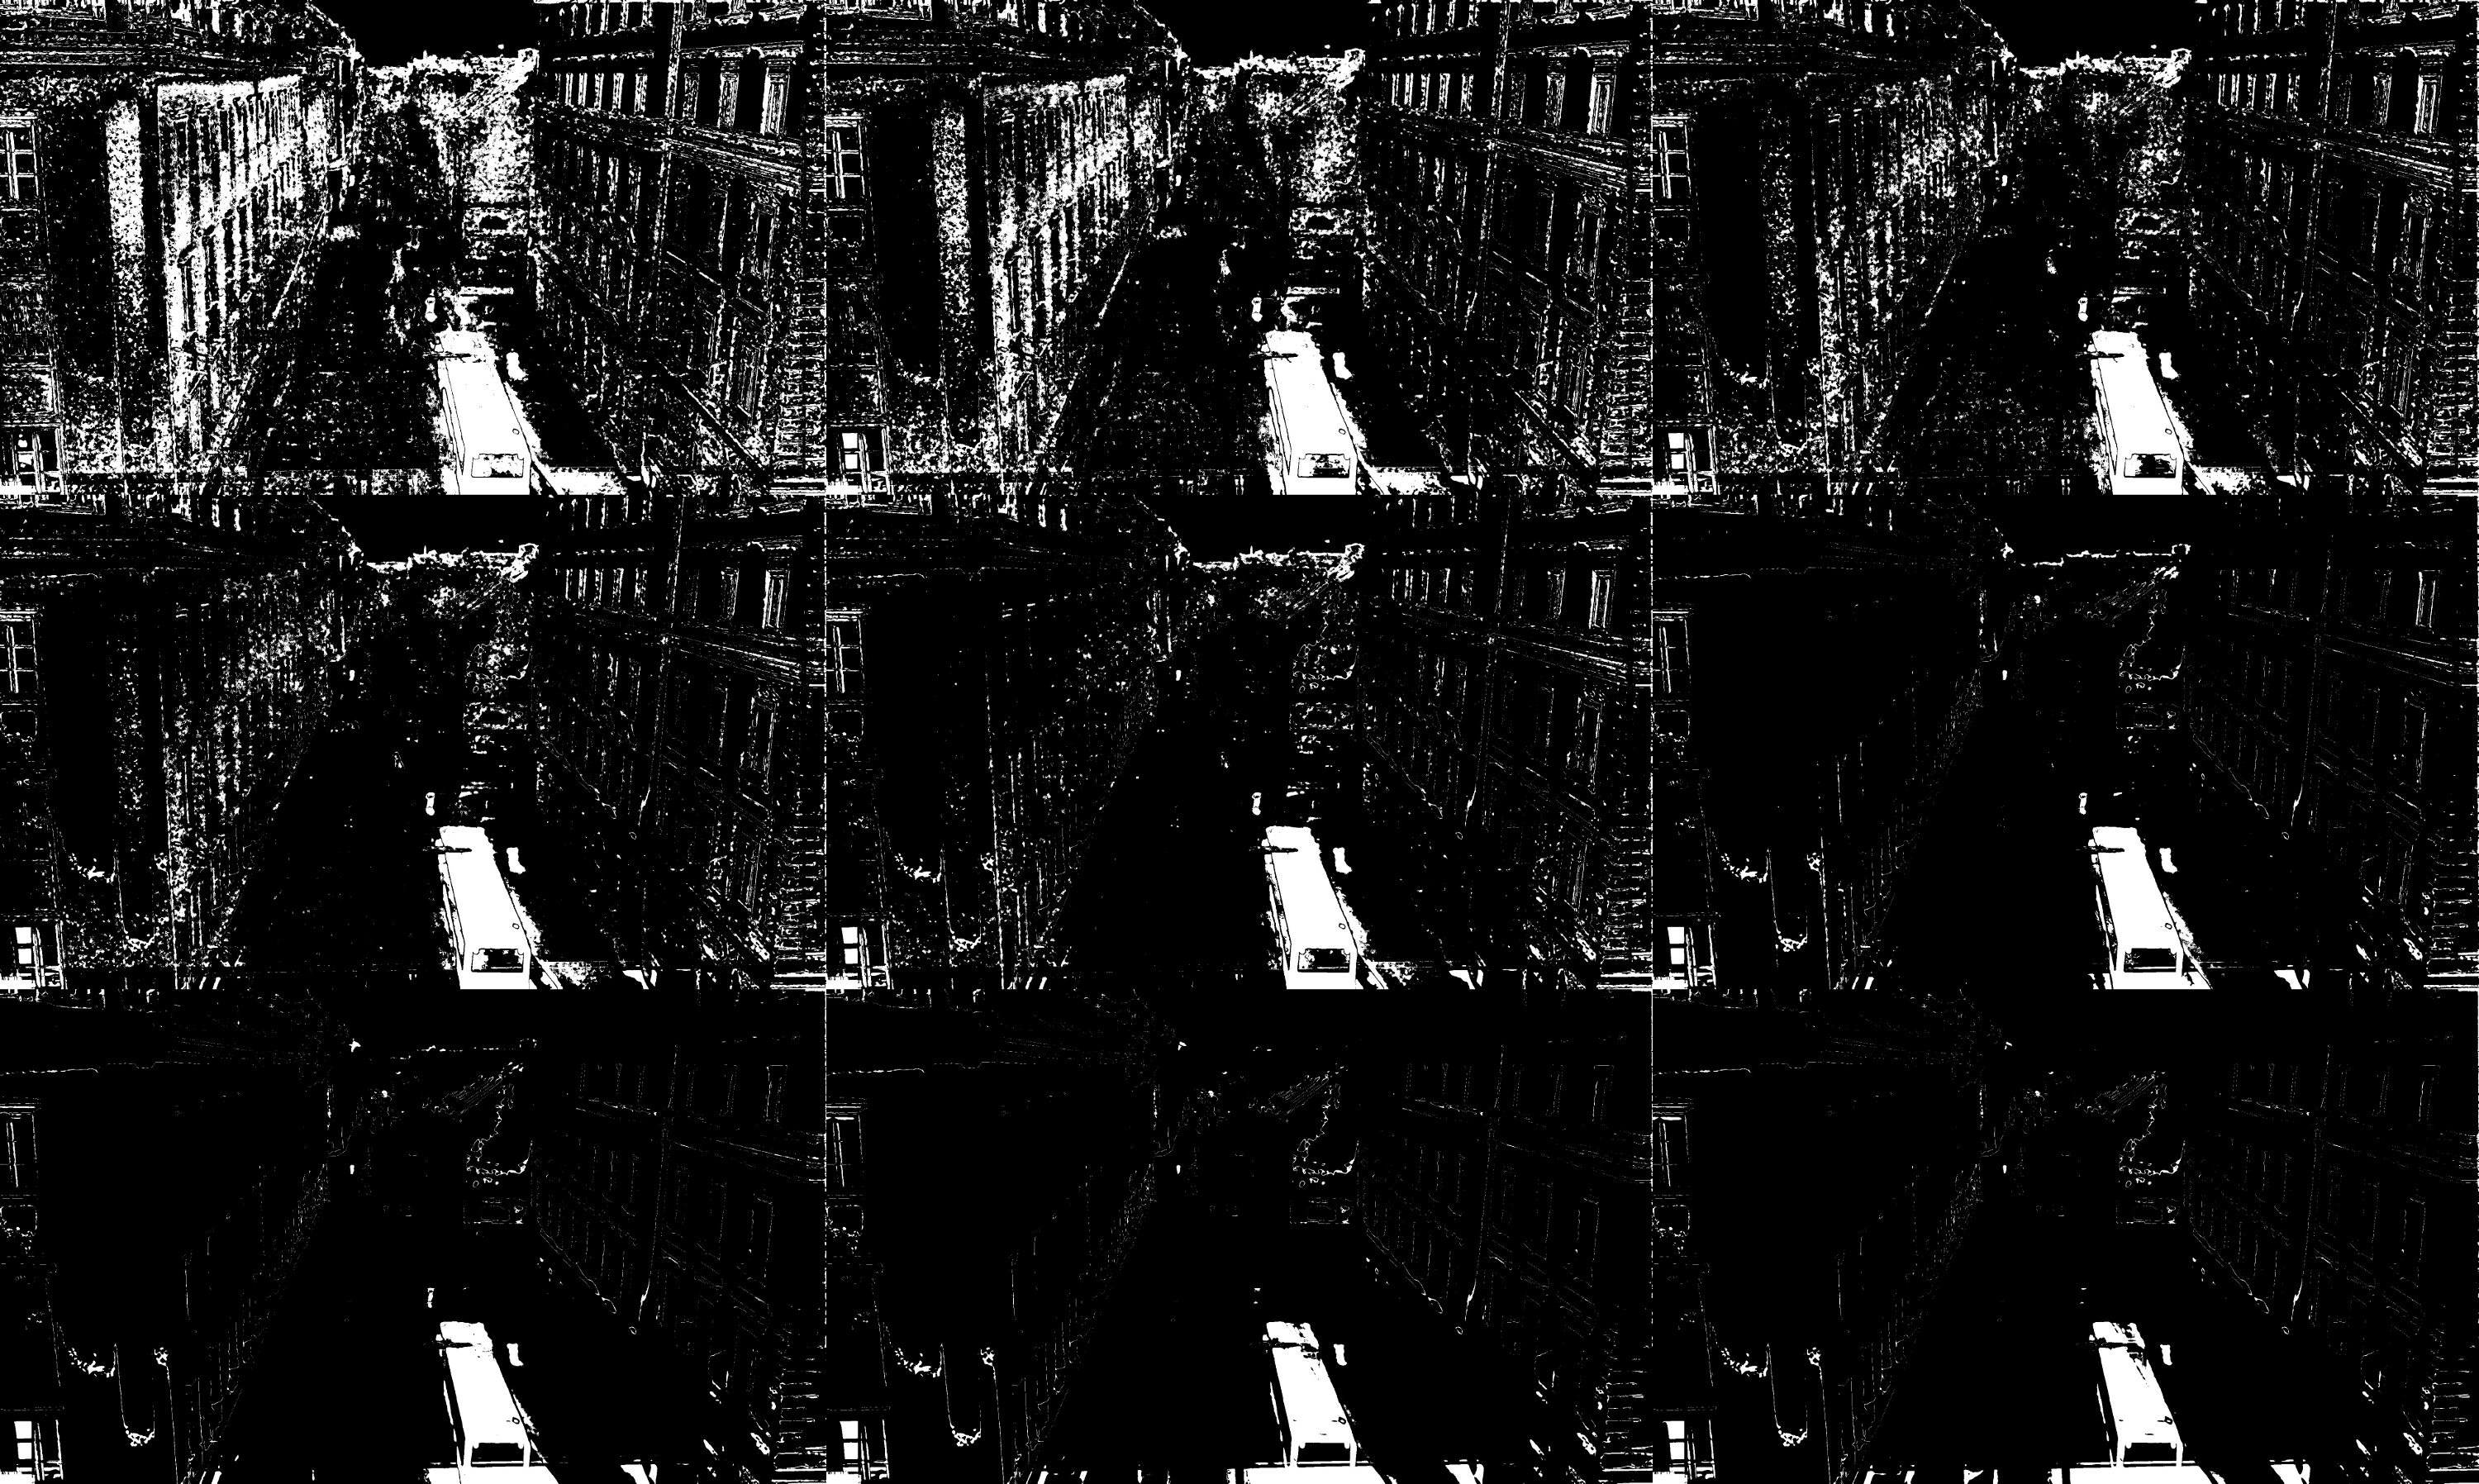
\includegraphics[scale = 0.14]{pics/alpha.jpg}
\caption{The influence of parameter $\alpha$ by increasing it}
\label{1}
\end{figure}


The results in the following figures show how nice the algorithm works although we're using only low-level pixel-wise operation by applying our algorithm on some main places in the city Graz (Austria).

\begin{figure}[h!t]
\centering
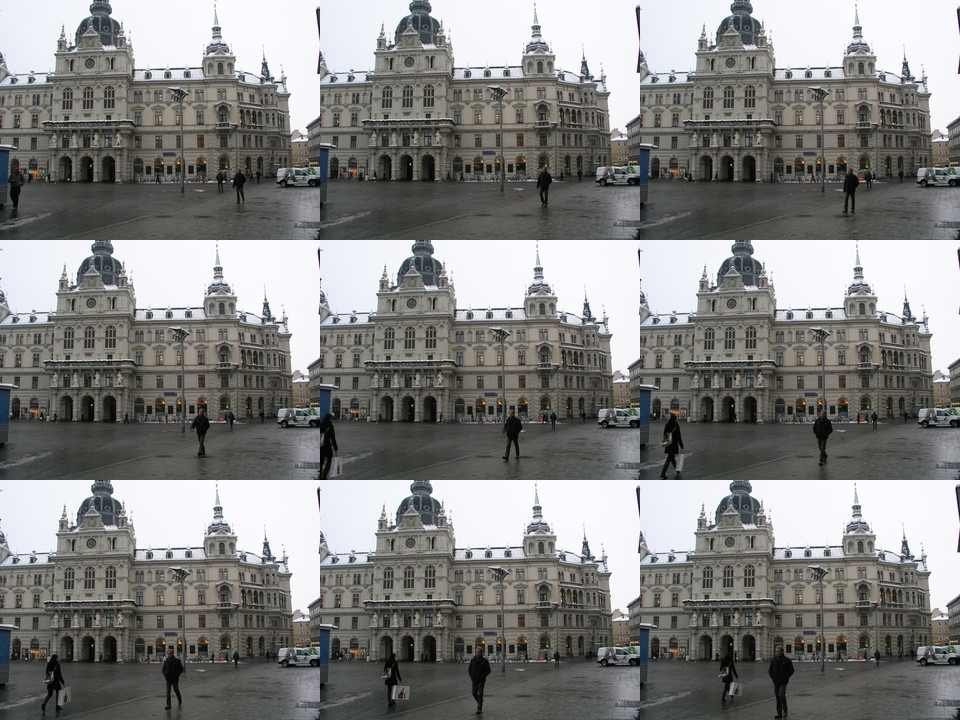
\includegraphics[scale = 0.43]{pics/rathaus.jpg}
\caption{Used input frames for "cleaning" the picture of the city hall in Graz}
\end{figure}

\begin{figure}[h!t]
\centering
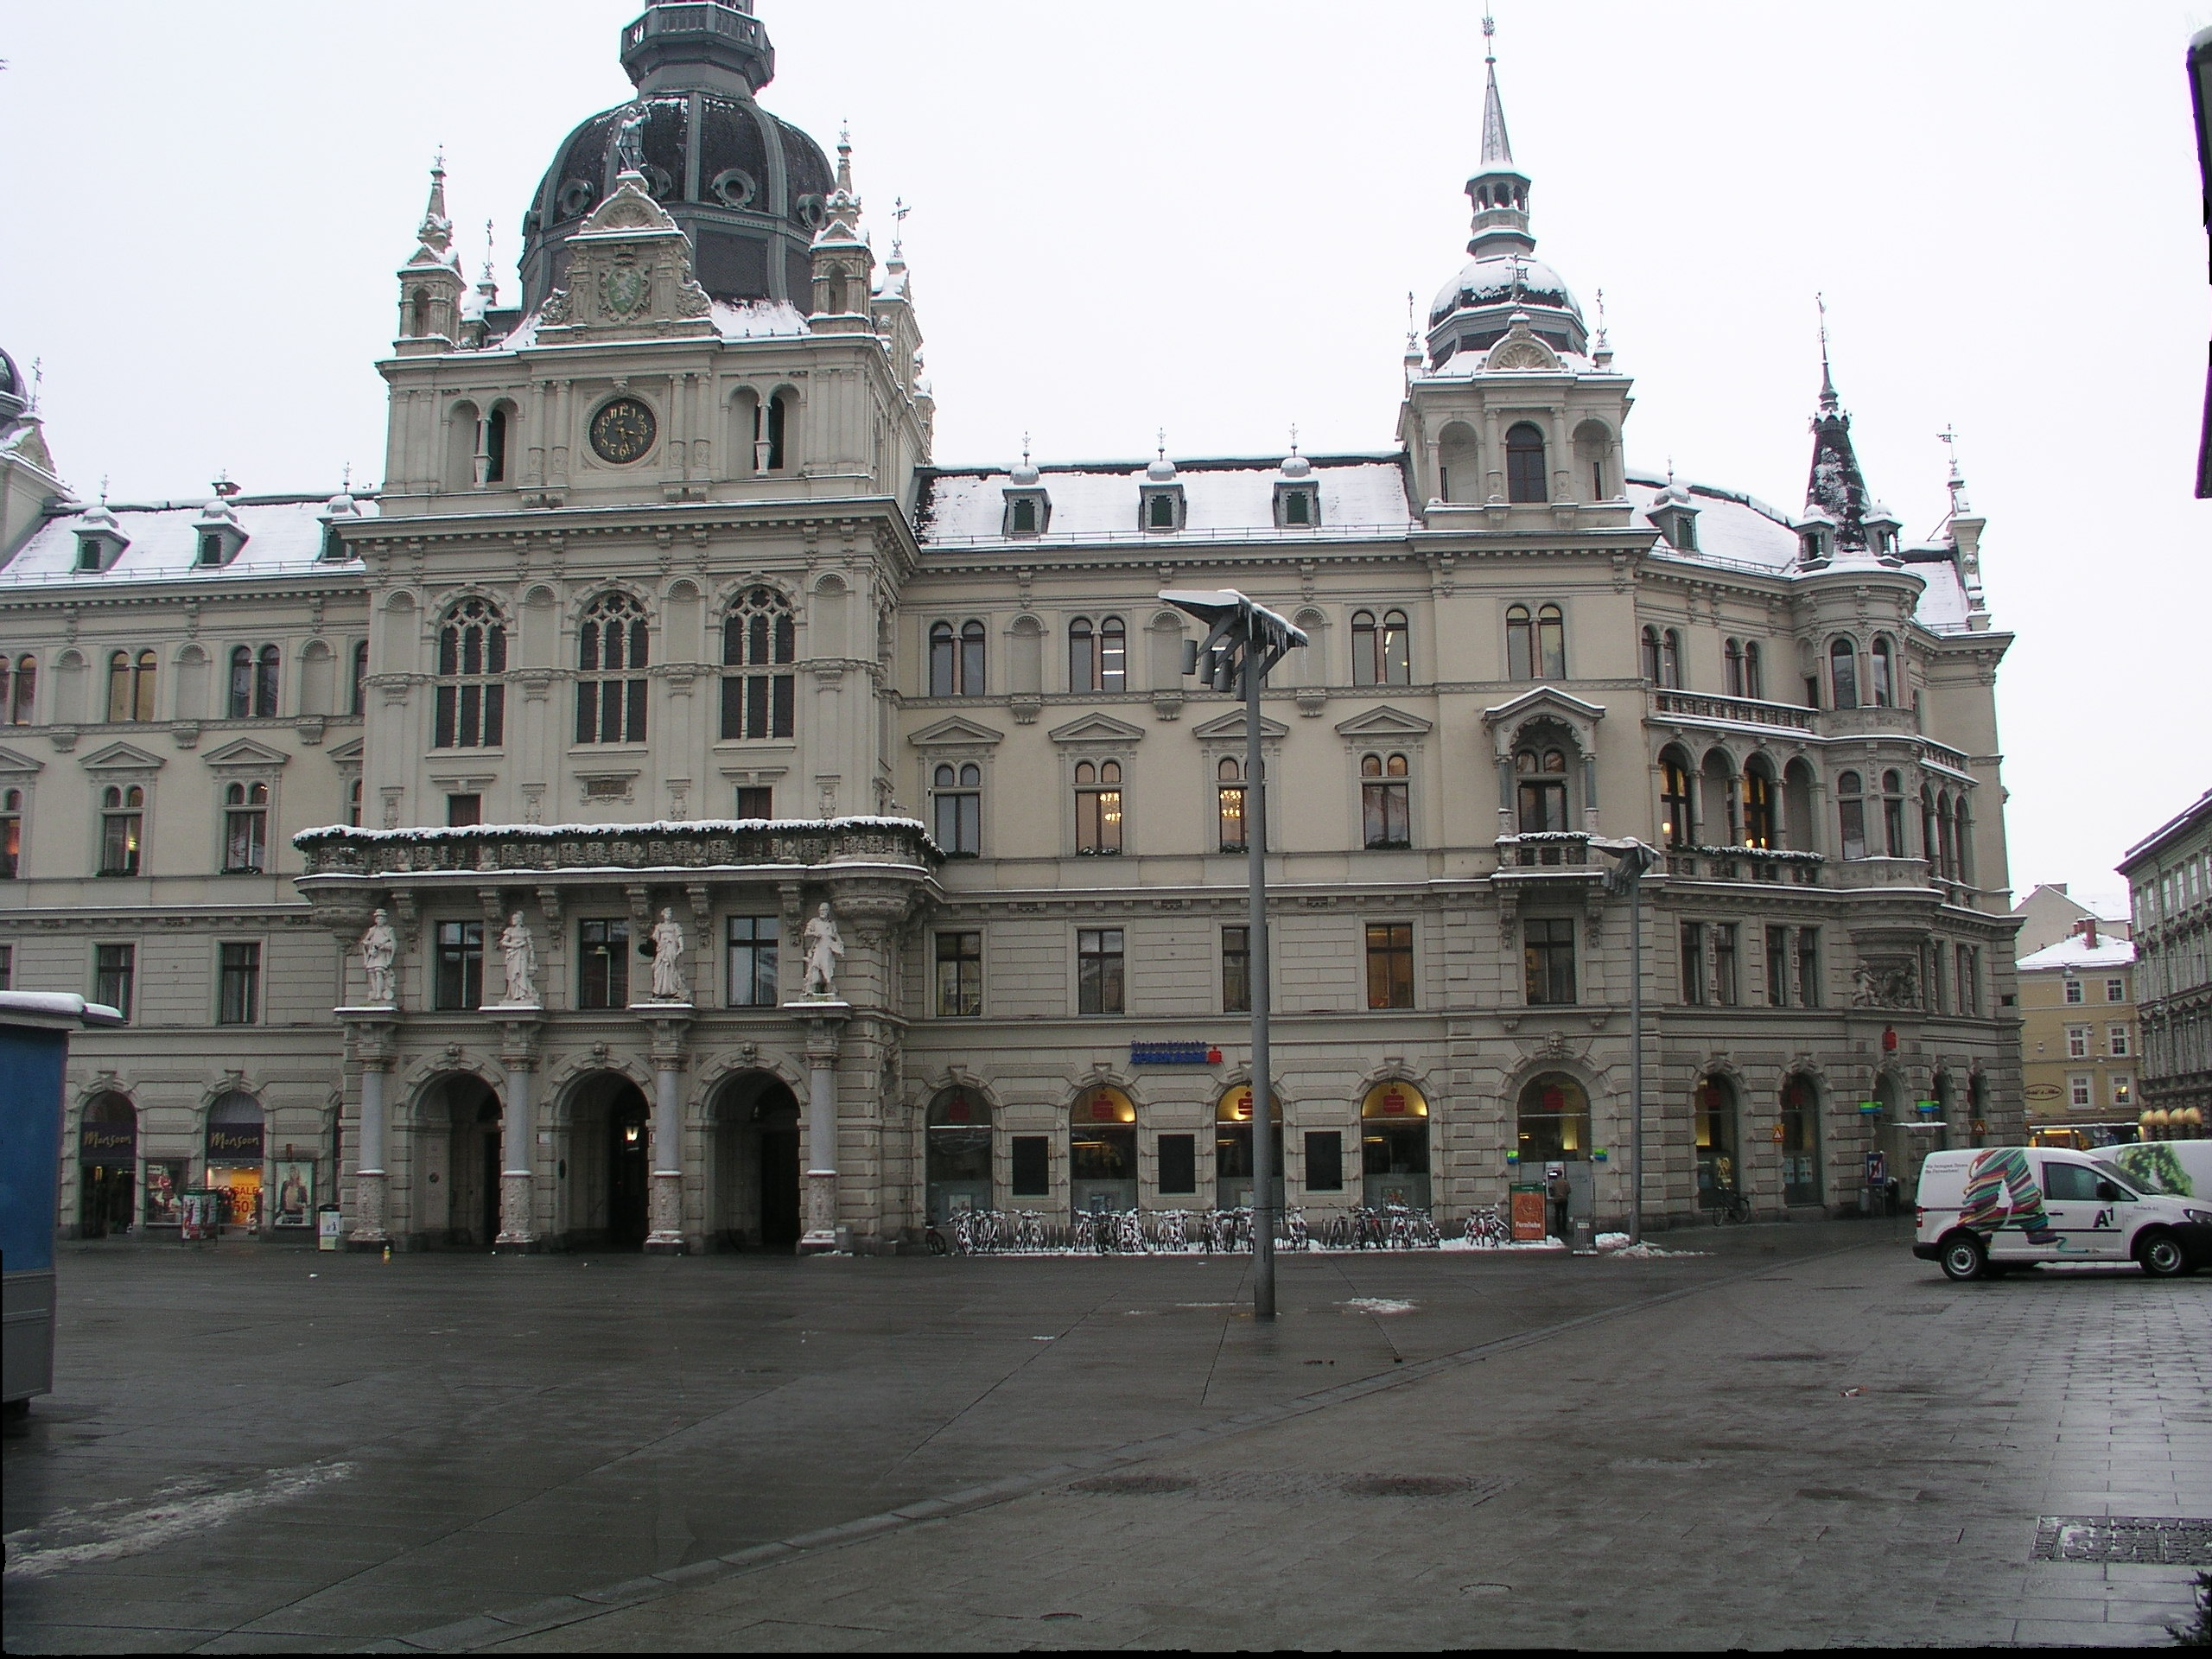
\includegraphics[scale = 0.16]{pics/result.jpg}
\caption{Resulting "cleaned" picture of the city hall of Graz}
\end{figure}

\newpage
As seen satisfiable results can be obtained. Furthermore an extreme test for the \textit{Jakominiplatz} in Graz was done with the following results:

\begin{figure}[h!t]
\centering
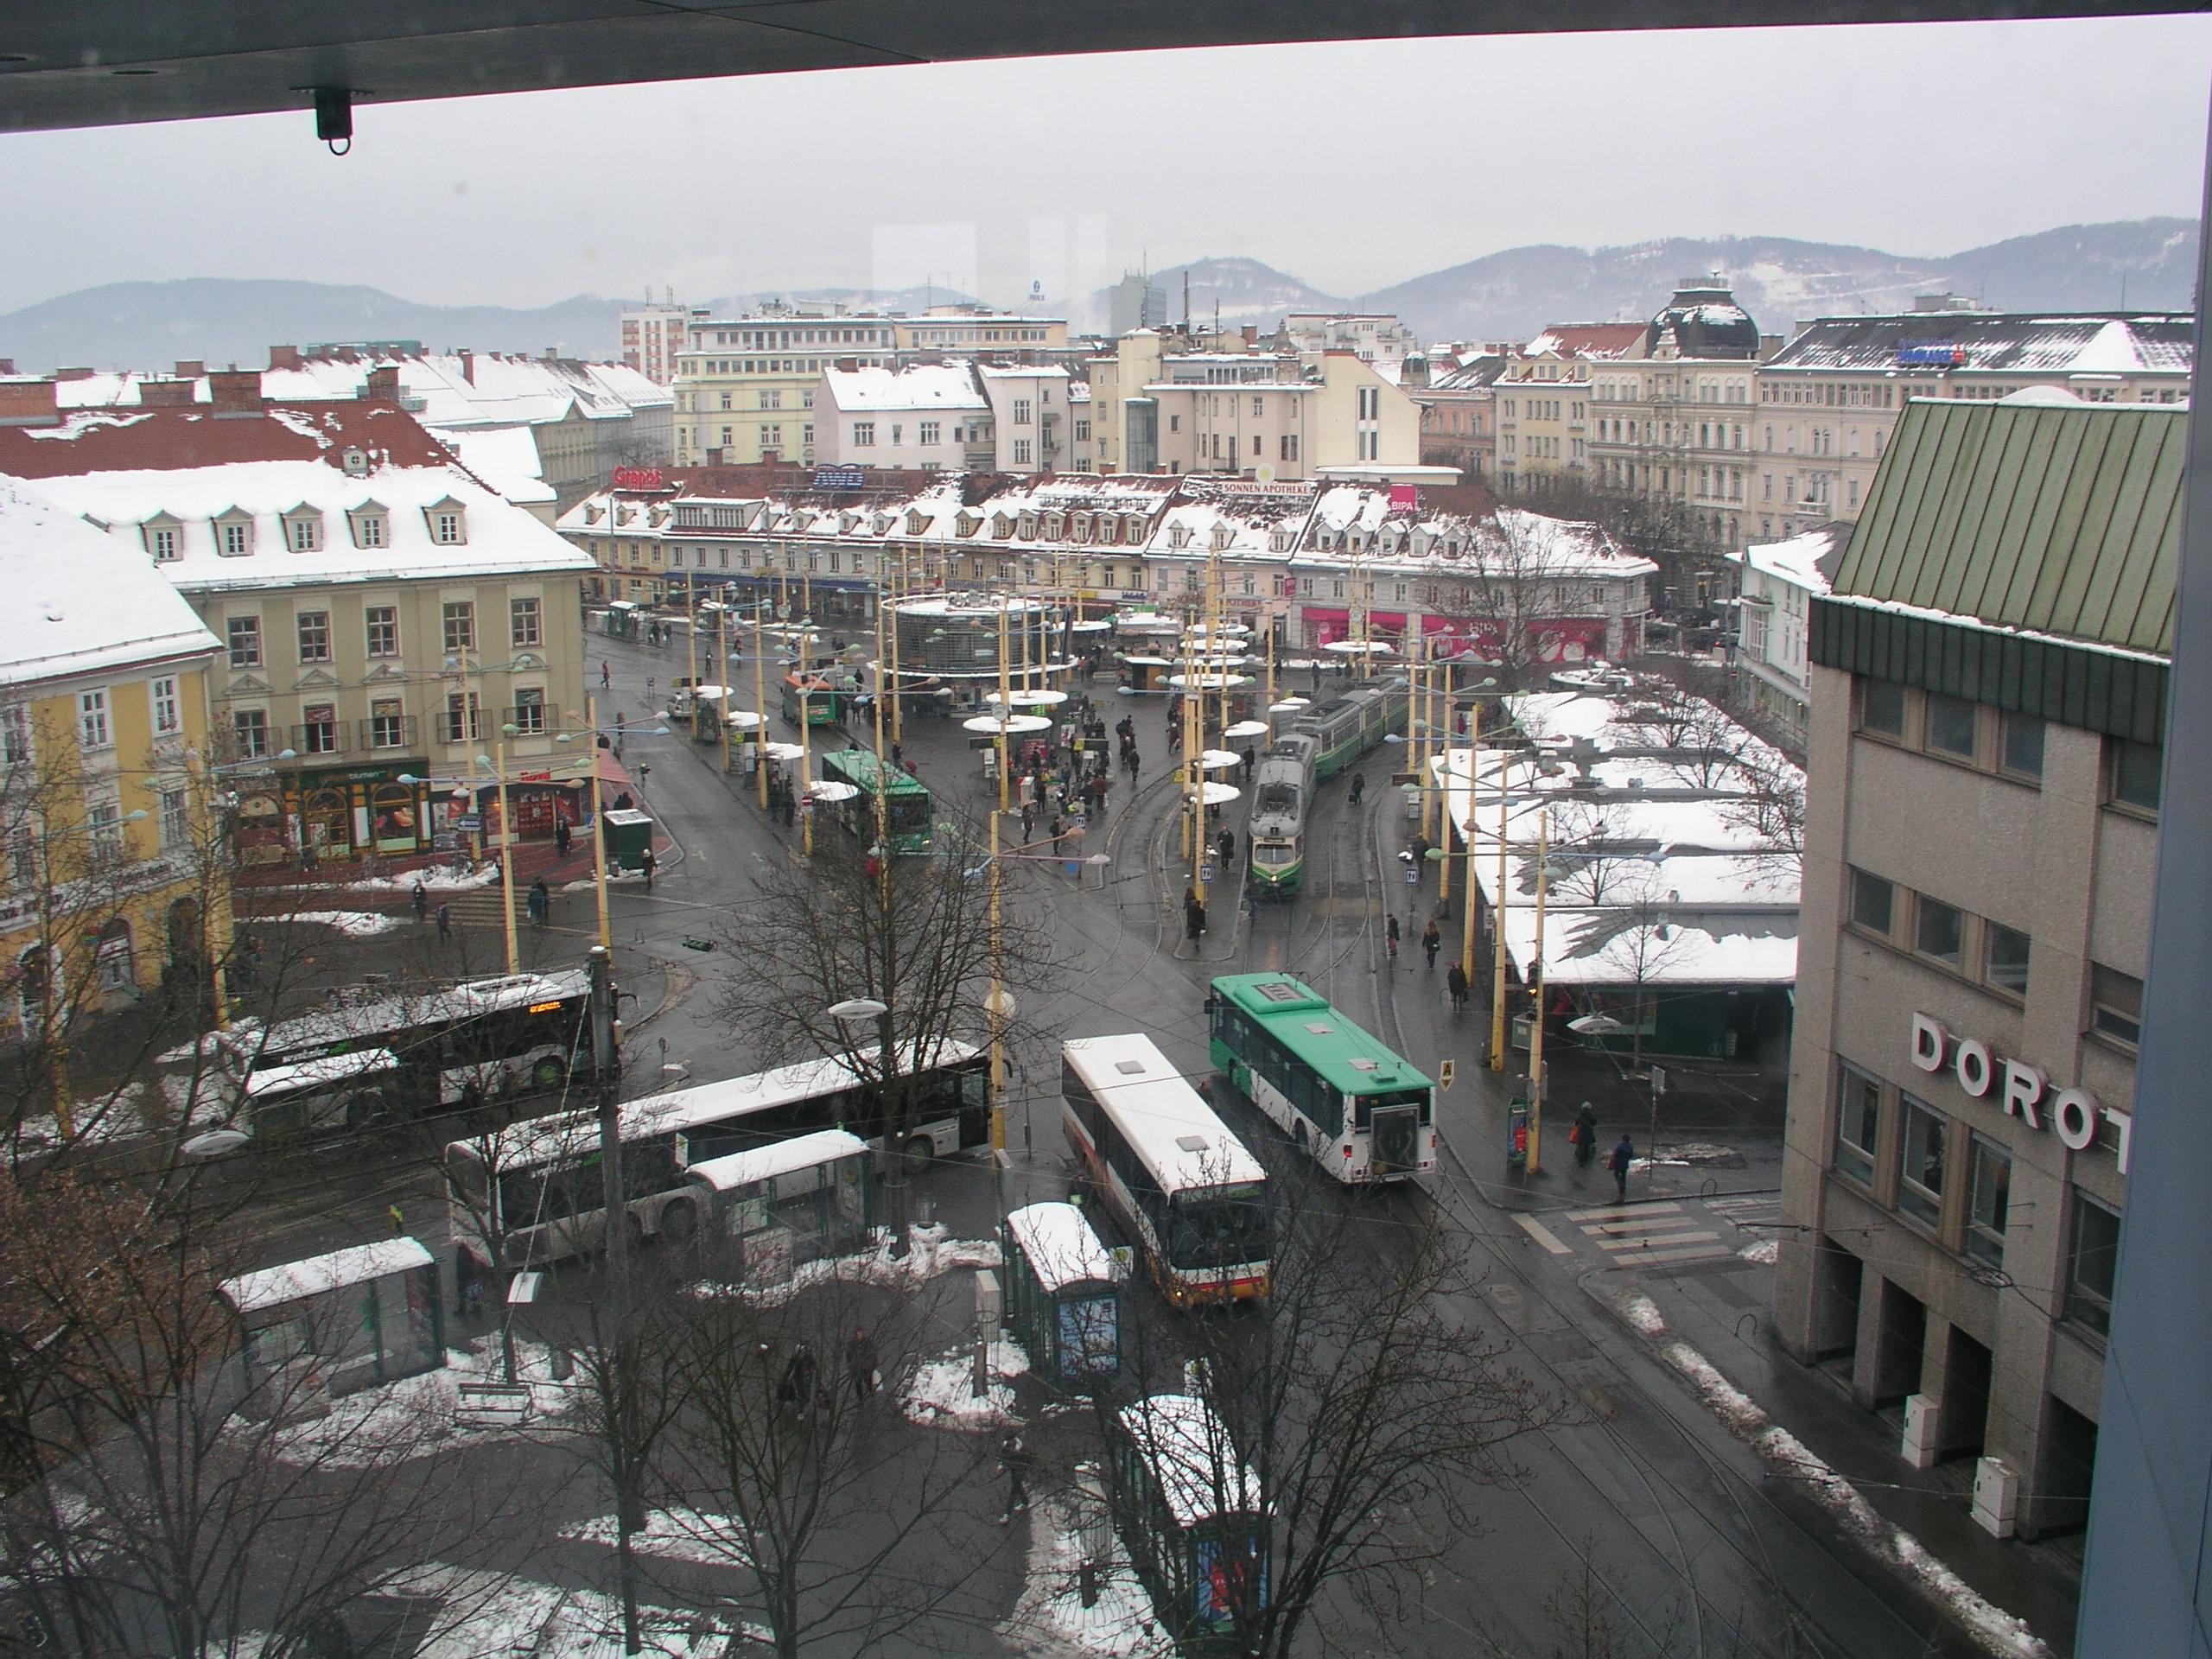
\includegraphics[scale = 0.145]{pics/jako_before.jpg}
\caption{Picture of the \textit{Jakominiplatz} of Graz}
\end{figure}

\begin{figure}[h!t]
\centering
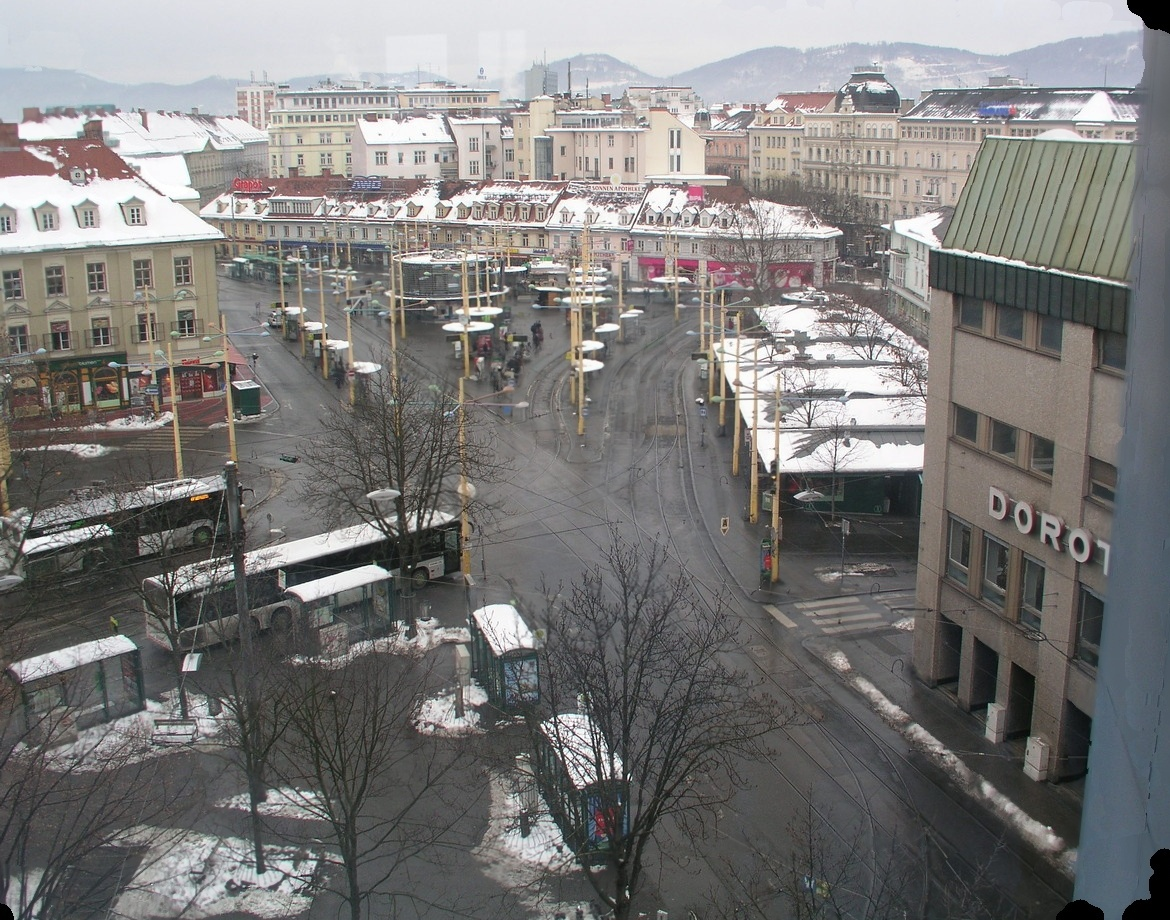
\includegraphics[scale = 0.32]{pics/jako.jpg}
\caption{Resulting "cleaned" picture of the \textit{Jakominiplatz} of Graz}
\end{figure}

Only "waiting" people and standing buses are still in the image..

\chapter{Discussion}

All in all the expected goal was achieved by our implementation as it can be seen in the result images.\\
Nevertheless some problems (which were not expected) did arise. The main problem was/is the in some kind inaccurate estimation of the homography for the image matching. This is a big problem if using pixelwise operations where especially the outer regions of the image are concerned.\\
The next point was to find an appropriate blending mechanism to fill the gaps of the foreground regions. Further we payed attention on the efficiency of our program which lead to more trade-offs between accuracy and speed.\\\\

The limits of our implementation is still dependent on the frequency of foreground such as persons moving through the scene. If many persons cover the background it is still impossible to do a reconstruction which becomes obvious because then also humans are not able to "see" behind obstacles.\\\\

To improve our algorithm we could add additional features for determining/evaluating the overall variance, such as gradient information or edge information. Besides that the neighborhood of each pixel could be included which may lead to more robustness and to better results.





%\chapter{Listings}


%\section{Simulation}
%\lstinputlisting[language=matlab]{bla}

%\section{Noise Cancelation}
%\lstinputlisting[language=matlab]{../matlab/3_4/m34.m}

%\section{Performancevergleich (N)LMS}
%\lstinputlisting[language=matlab]{../implementation/lms_performance.m}


% **************************************************************************************************
% **************************************************************************************************

%\appendix
%\bibliographystyle{/.base/ieeetran}
%\bibliography{_bibliography}

% place all floats and create label on last page
\FloatBarrier\label{end-of-document}
\end{document}

